\documentclass[main.tex]{subfiles}
\begin{document}

\section{Photon statistics}


\begin{figure}[ht]
\centering


\tikzset{every picture/.style={line width=0.75pt}} %set default line width to 0.75pt        

\begin{tikzpicture}[x=0.75pt,y=0.75pt,yscale=-1,xscale=1]
%uncomment if require: \path (0,300); %set diagram left start at 0, and has height of 300

%Shape: Rectangle [id:dp22021547584457224] 
\draw   (32,82) -- (102,82) -- (102,122) -- (32,122) -- cycle ;
%Shape: Wave [id:dp04968334570050592] 
\draw  [dash pattern={on 4.5pt off 4.5pt}] (103,100.7) .. controls (107.08,104.03) and (110.98,107.2) .. (115.5,107.2) .. controls (120.02,107.2) and (123.92,104.03) .. (128,100.7) .. controls (132.08,97.37) and (135.98,94.2) .. (140.5,94.2) .. controls (145.02,94.2) and (148.92,97.37) .. (153,100.7) .. controls (157.08,104.03) and (160.98,107.2) .. (165.5,107.2) .. controls (170.02,107.2) and (173.92,104.03) .. (178,100.7) .. controls (182.08,97.37) and (185.98,94.2) .. (190.5,94.2) .. controls (195.02,94.2) and (198.92,97.37) .. (203,100.7) .. controls (207.08,104.03) and (210.98,107.2) .. (215.5,107.2) .. controls (220.02,107.2) and (223.92,104.03) .. (228,100.7) .. controls (232.08,97.37) and (235.98,94.2) .. (240.5,94.2) .. controls (245.02,94.2) and (248.92,97.37) .. (253,100.7) .. controls (257.08,104.03) and (260.98,107.2) .. (265.5,107.2) .. controls (270.02,107.2) and (273.92,104.03) .. (278,100.7) .. controls (282.08,97.37) and (285.98,94.2) .. (290.5,94.2) .. controls (295.02,94.2) and (298.92,97.37) .. (303,100.7) .. controls (307.08,104.03) and (310.98,107.2) .. (315.5,107.2) .. controls (319.02,107.2) and (322.16,105.28) .. (325.3,102.86) ;
%Shape: Ellipse [id:dp2897372001959284] 
\draw   (354.86,88.89) .. controls (365.17,99.2) and (368.73,112.35) .. (362.82,118.27) .. controls (356.9,124.18) and (343.75,120.62) .. (333.44,110.31) .. controls (323.13,100) and (319.57,86.85) .. (325.48,80.93) .. controls (331.4,75.02) and (344.55,78.58) .. (354.86,88.89) -- cycle ;
%Shape: Wave [id:dp798169784205734] 
\draw  [dash pattern={on 4.5pt off 4.5pt}] (338.58,118.55) .. controls (335.34,122.64) and (332.25,126.55) .. (332.27,131.08) .. controls (332.29,135.6) and (335.4,139.49) .. (338.67,143.55) .. controls (341.95,147.62) and (345.06,151.5) .. (345.08,156.03) .. controls (345.09,160.55) and (342.01,164.46) .. (338.77,168.55) .. controls (335.53,172.64) and (332.45,176.55) .. (332.46,181.08) .. controls (332.48,185.6) and (335.59,189.49) .. (338.87,193.55) .. controls (342.14,197.61) and (345.25,201.5) .. (345.27,206.03) .. controls (345.28,208.94) and (344.01,211.6) .. (342.23,214.21) ;
%Shape: Chord [id:dp4480069197470371] 
\draw   (378.22,209.27) .. controls (380.01,212.87) and (381,216.84) .. (381,221) .. controls (381,237.57) and (365.33,251) .. (346,251) .. controls (326.67,251) and (311,237.57) .. (311,221) .. controls (311,216.84) and (311.99,212.87) .. (313.78,209.27) -- cycle ;

% Text Node
\draw (40,93) node [anchor=north west][inner sep=0.75pt]   [align=left] {LASER};
% Text Node
\draw (316,218) node [anchor=north west][inner sep=0.75pt]   [align=left] {Detector};
% Text Node
\draw (292,51) node [anchor=north west][inner sep=0.75pt]   [align=left] {Sandpaper disk};


\end{tikzpicture}
\caption{Sandpaper setup.}
\label{fig:sandpaper}
\end{figure}

\subsection{Analysis}

With the sandpaper disk kept stationary, we expect the coherent state of the laser to be preserved, and therefore to have 
%
\begin{align}
\mathbb{P} (n) = \frac{e^{-\overline{n}} \overline{n}^{n}}{n!}
\,,
\end{align}
%
while if the sandpaper disk is rotating we expect to see a thermal distribution, with 
%
\begin{align}
\mathbb{P} (n) = \frac{\overline{n}^{n}}{(1 + \overline{n})^{n+1}}
\,.
\end{align}

In order to see how these theoretical distributions compare to the data, we compute their first moments: the mean 
%
\begin{align}
\overline{n} = \sum _{n} \mathbb{P}(n) n
\,,
\end{align}
%
the variance 
%
\begin{align}
\sigma^2 = \sum _{n} \mathbb{P}(n) (n - \overline{n})^2
\,,
\end{align}
%
the normalized skewness 
%
\begin{align}
\text{skewness} = \frac{1}{\sigma^3} \sum _{n} \mathbb{P}(n) (n - \overline{n})^3
\,,
\end{align}
%
and the normalized kurtosis 
%
\begin{align}
\text{kurtosis} = \frac{1}{\sigma^4} \sum _{n} \mathbb{P}(n) (n - \overline{n})^4
\,.
\end{align}

The only parameter the distributions depend on is the mean; so starting from it we compute these moments. 
The results, for window sizes varying from \SI{10}{ns} to approximately \SI{3}{ms}, are shown in figure \ref{fig:photon_statistics}.

\begin{sidewaysfigure}[ht]
    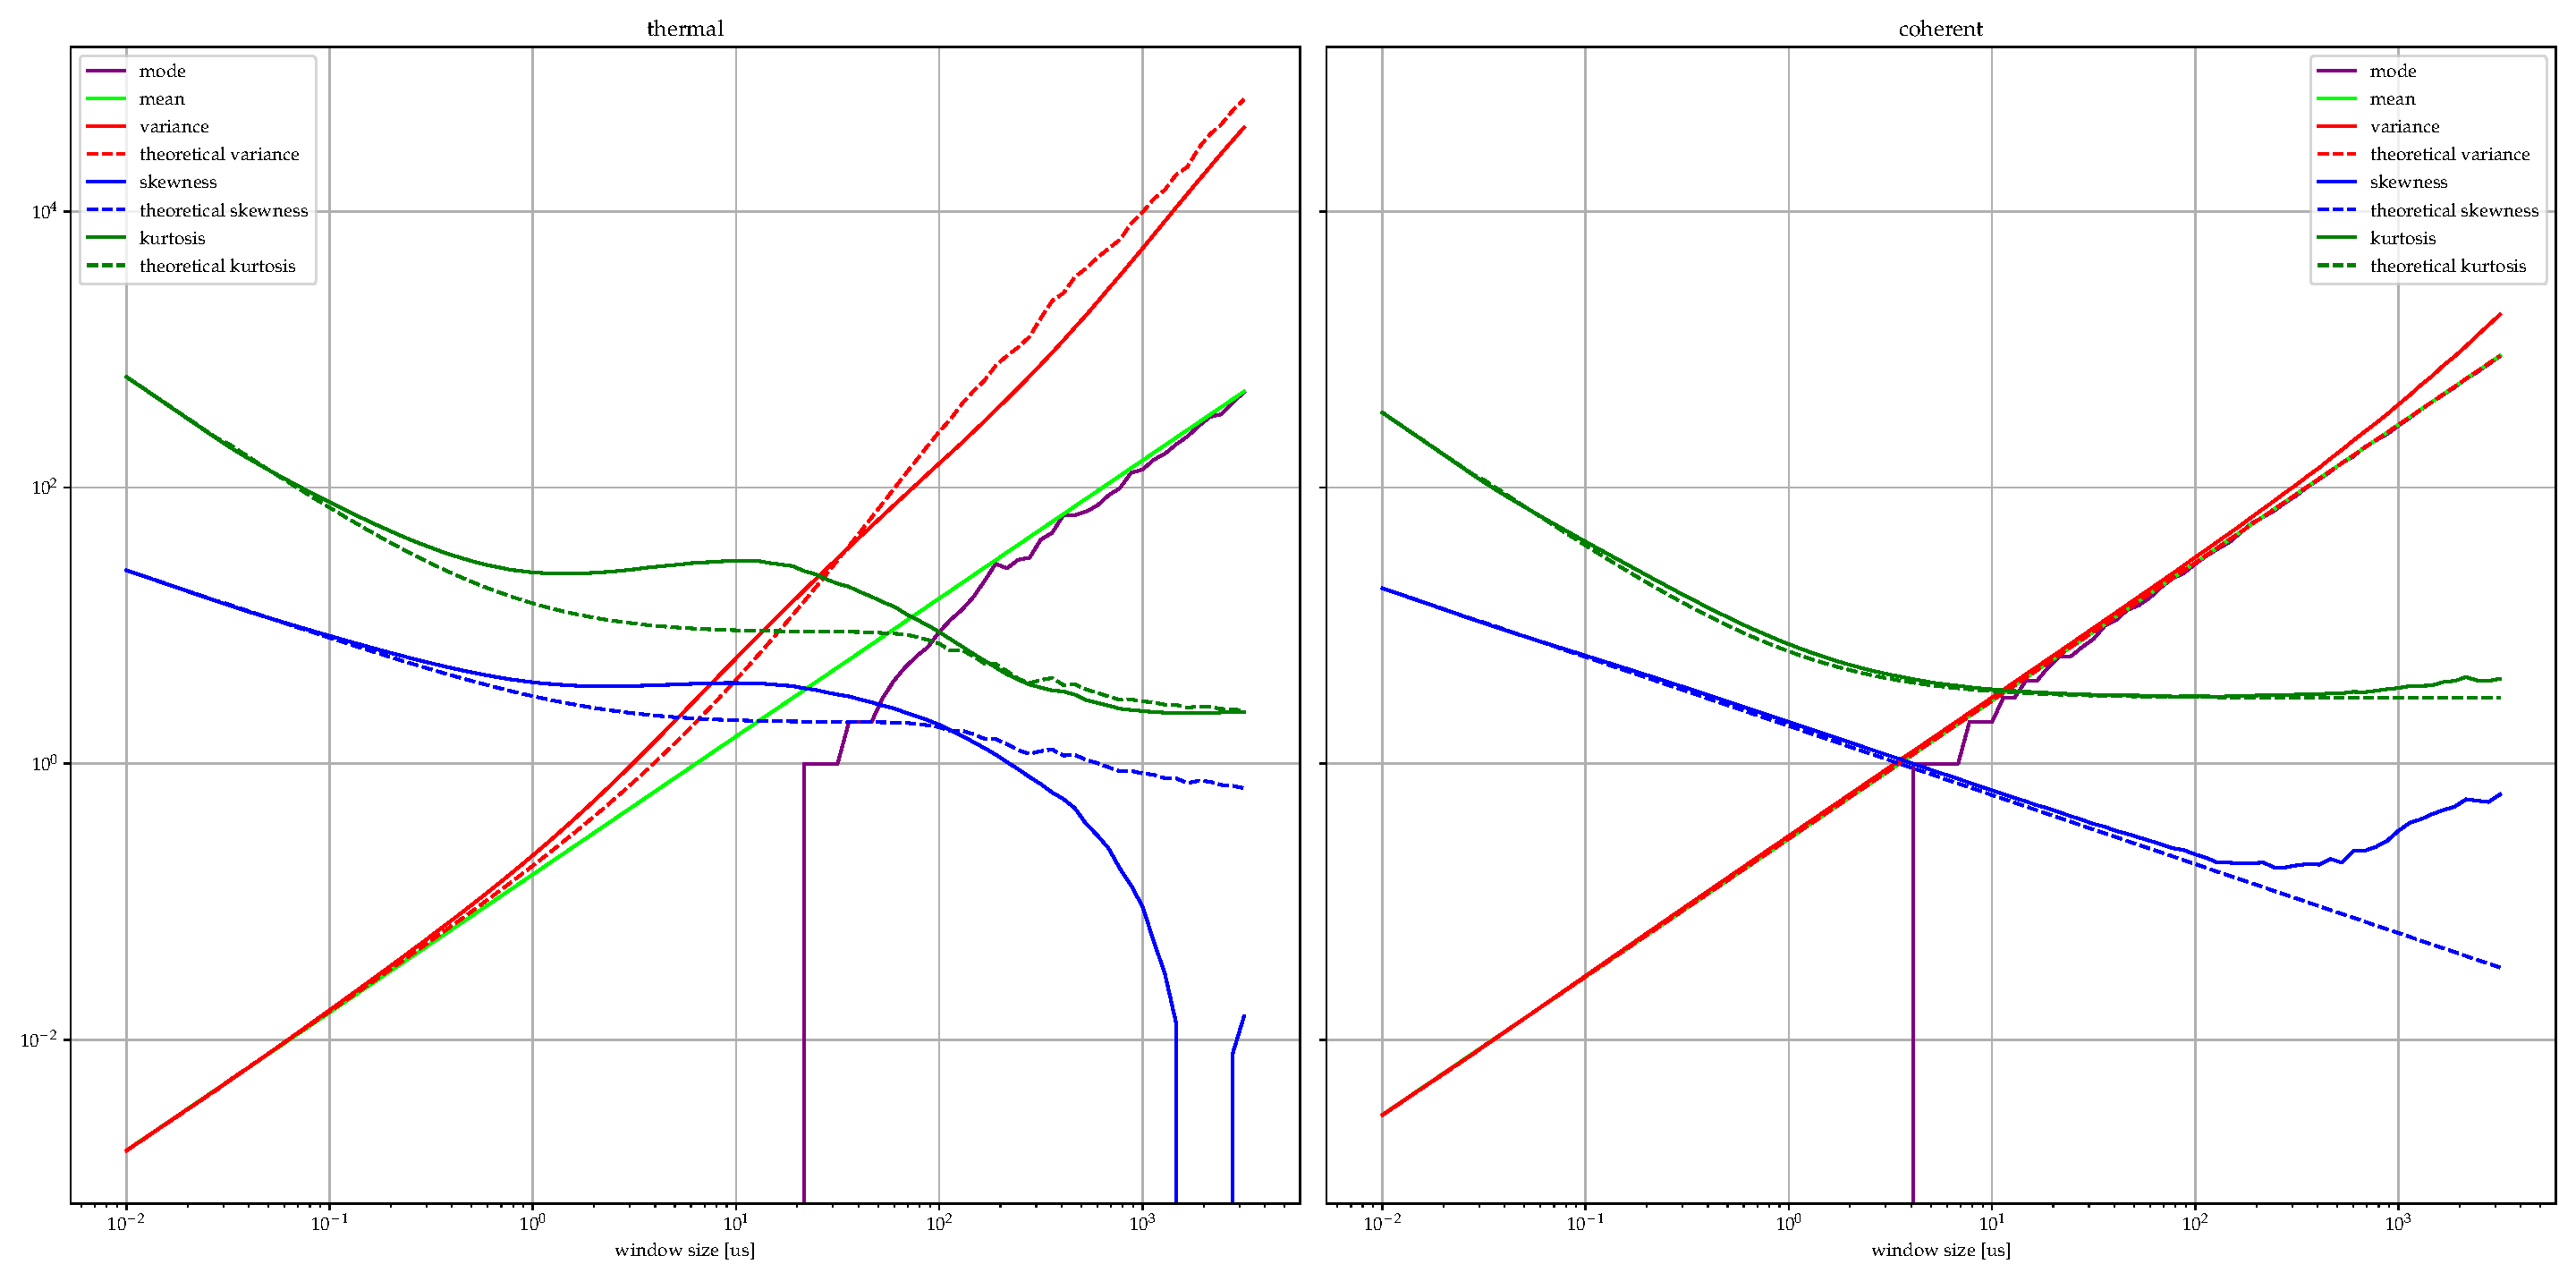
\includegraphics[width=\textwidth]{figures/photon_statistics.pdf}
    \caption{Photon statistics.}
    \label{fig:photon_statistics}
\end{sidewaysfigure}

\end{document}